\begin{figure}[t]
\centering
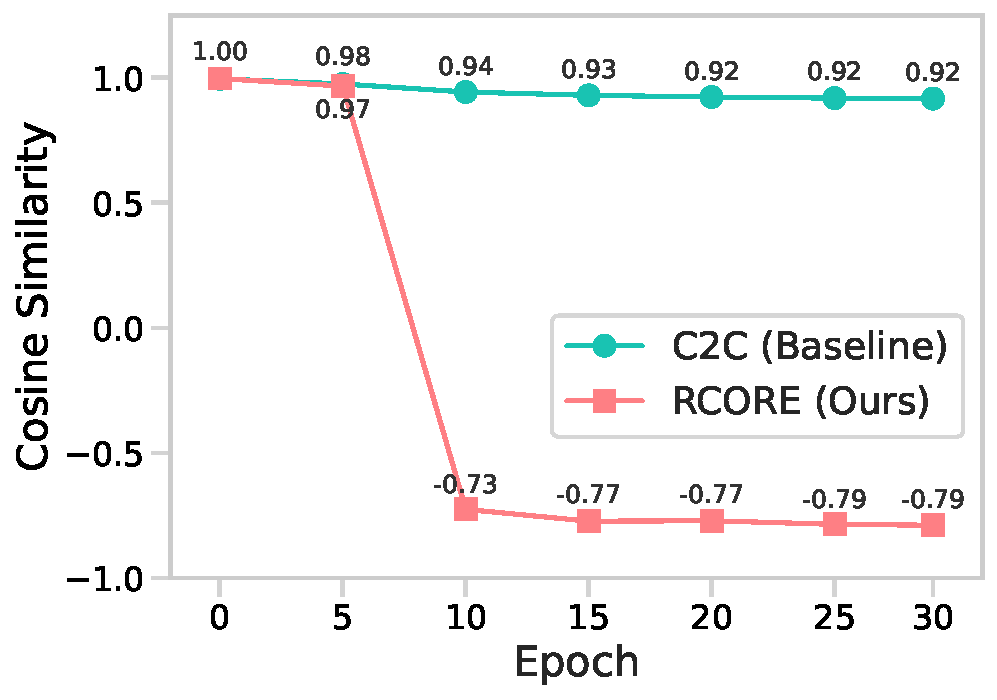
\includegraphics[width=.5\linewidth]{figure/supple_src/cosine_loss_clip.pdf}
\vspace{-1em}
\figcapmargin
\figcaption{Similarity analysis between original and reversed verb features}{
    We plot the cosine similarity between the original and reversed verb features for the baseline (C2C~\cite{li2024c2c}) and \ours{} with the CLIP~\cite{radford2021clip} backbone on the Sth-com~\cite{li2024c2c} dataset.
    The baseline maintains a \textit{high similarity} (+0.92) during entire training, revealing limited temporal sensitivity.
    In contrast, the similarity becomes \textit{strongly negative} for \ours{} as training progresses, indicating improved temporal discriminative capability.
}
\label{fig:cosine_sim}
\end{figure}



